\begin{remark}
    Section made from lectures done by Jøran Moen. Other sources are \citet{1995Itsp} --- chapter 2.
\end{remark}

\section{Single particle motion}
\subsection{Gyro-motion}
We first look at the motion of single particles. From the equation of motion we have
\begin{equation*}
    m\frac{\text{d}\gf{v}}{\text{d}t}=q\gf{E}+\underbrace{q\gf{v}\times\gf{B}}_{\text{Lorentz}}+\cancelto{0}{m\gf{g}}
\end{equation*}
If we look at motion due to the magnetic field, the gyro-motion (cyclotron), we let \(\gf{E}=\gf{0}\), leaving only the magnetic field from the equation above, hence we get
\begin{equation*}
    m\frac{\text{d}{\gf{v}}}{\text{d}t}=q\gf{v}\times\gf{B}
\end{equation*}
\begin{align*}
    m\frac{\text{d}\gf{v}}{\text{d}t}&=q\gf{v}_\perp\times\gf{B}\\
    &=m\gf{a}_\perp=\frac{\gf{v}_\perp^2}{r_c}m\Rightarrow r_c=\frac{\gf{v}_\perp^2}{\gf{a}_\perp}=\frac{m\gf{v}_\perp}{q\gf{B}}
\end{align*}
So the only acceleration we have is the acceleration perpendicular to the magnetic field lines. The equation above describes gyro-motion, and the period of one gyration is
\begin{equation*}
    \tau_c=\frac{2\pi m}{qB}
\end{equation*}
with angular frequency
\begin{equation*}
    \omega_c=\frac{qB}{m}
\end{equation*}
\begin{figure}[t]
    \centering
    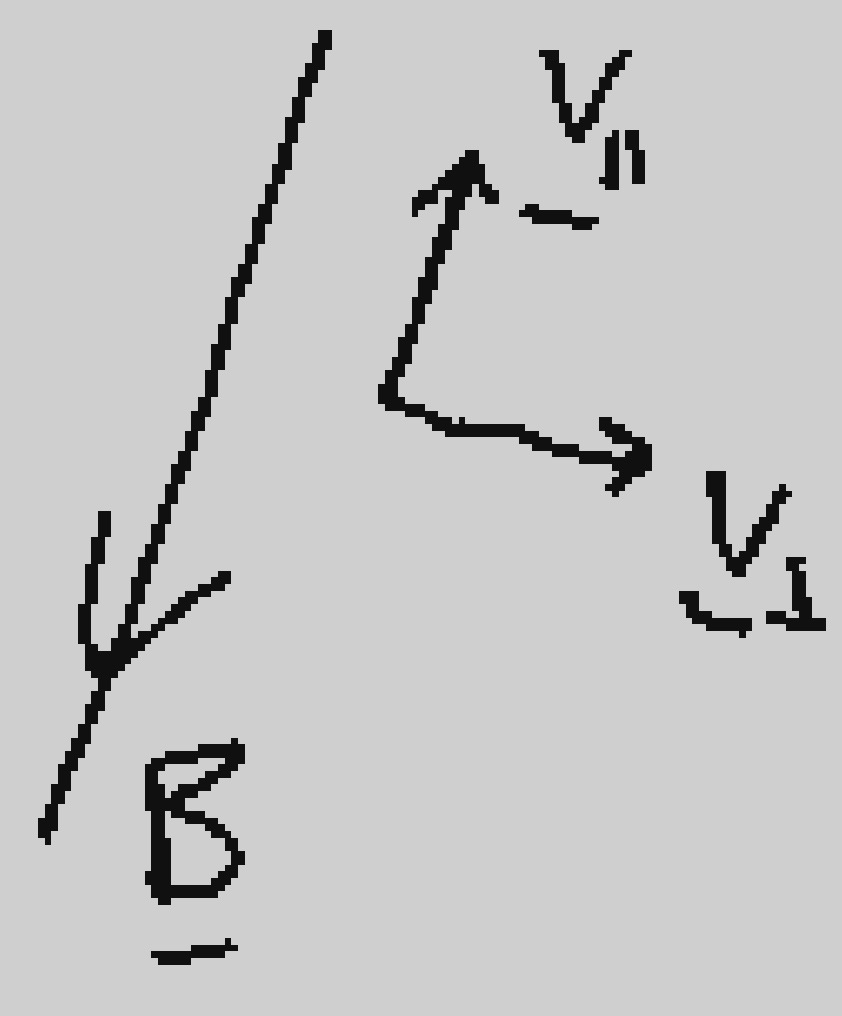
\includegraphics[width=.15\linewidth]{bilder/v_decomp.jpg}\label{fig:v_decomp}
    \caption{Graphical description of the definition of parallel and perpendicular directions.}
\end{figure}

\subsection{\(\gf{E}\times\gf{B}\)-drift}
We first want to look at the \(\orderof(0)\) of the motion of the single particles. We look at the parallel and perpendicular components individually. \boxed{\vert\vert:}
\begin{equation*}
    m\frac{\text{d}\gf{v}}{\text{d}t}=\gf{F}_{\vert\vert}=q\gf{a}_{\vert\vert}=0
\end{equation*}
\boxed{\perp:}
\begin{equation*}
    m\frac{\text{d}\gf{v}}{\text{d}t}=\gf{F}_\perp=q\gf{a}_\perp=0
\end{equation*}
\begin{figure}[t]
    \centering
    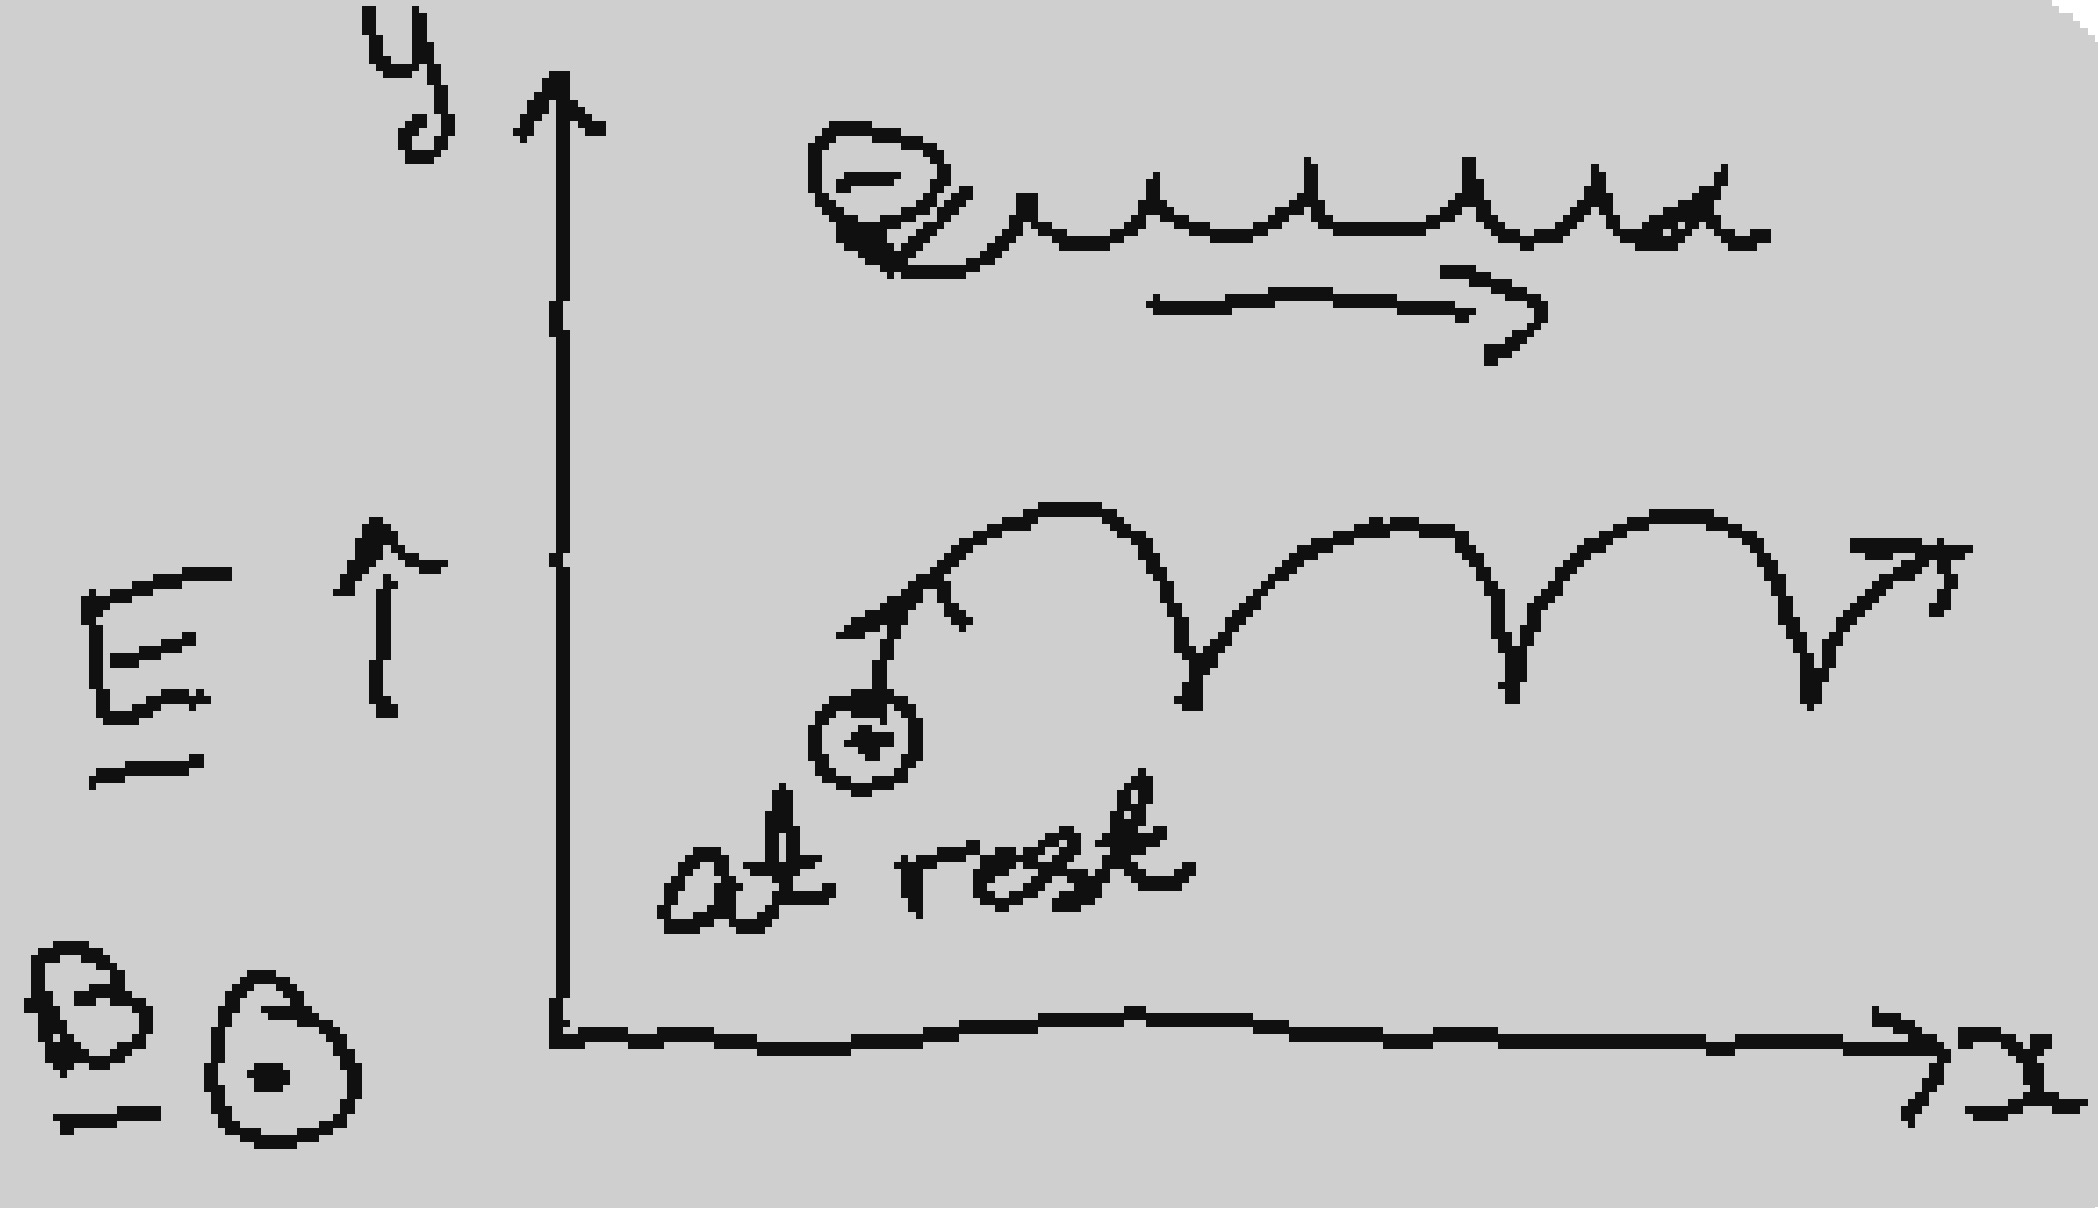
\includegraphics[width=0.2\linewidth]{bilder/ExB.jpg}\label{fig:ExB}
    \caption{\(\gf{E}\times\gf{B}\)-drift of ions and electrons.}
\end{figure}
We want to look at the drift we get from the \(E\)- and \(B\)-fields when they have perpendicular components. Let \(\gf{v}_\perp=\gf{u}_E+\gf{v}_\perp'\) where \(\gf{u}_E\) describe the constant motion and \(\gf{v}'\) describe accelerated motion.
\begin{align*}
    \Rightarrow m\frac{\text{d}\gf{v}'}{\text{d}t}+\cancelto{0}{m\fracdt{\gf{u}_E}}&=q\gf{E}_\perp+q\gf{v}'\times\gf{B}+q\gf{u}_E\times\gf{B}\\
    \underbrace{m\fracdt{\gf{v}'}-q\gf{v}'\times\gf{B}}_{\substack{=0 \textnormal{ when avg} \\\textnormal{over one period}}}&=q\gf{E}_\perp+q\gf{u}_E\times\gf{B}\quad\vert\times\gf{B}\\
    \gf{E}_\perp\times\gf{B}&=\gf{u}_{E}B^2-\gf{B}\cancelto{0}{(\gf{B}\cdot\gf{u}_E)}
\end{align*}
\begin{equation*}
    \therefore \gf{u}_E=\frac{\gf{E}\times\gf{B}}{B^2}
\end{equation*}
This generalizes to
\begin{equation}\label{eq:gen_v_drift}
    \gf{u}_F=\frac{\gf{F}\times\gf{B}}{qB^2}
\end{equation}

\subsection{\(\nabla\gf{B}\)-drift}
We linearize the magnetic parameter, i.e.\ we let \(\gf{B}=\gf{B}_0+(\partial_y\gf{B})y\f{z}+\orderof(2)\) where we assume the second order terms are negligible and where \(\gf{B}=B\f{z}\).
\begin{equation*}
    \gf{F}_x=qv_{y}B
\end{equation*}
\begin{align*}
    \gf{F}_y=-qv_{x}B&=m\dot{v}_y,\qquad\text{int.\ w.r.t } t\\
    mv_y=-qxB&=-qr_c\sin(\phi)B
\end{align*}
\coloredeqq{\Rightarrow{} v_y=-v_\perp\sin(\phi),\quad v_x=v_\perp\cos(\phi)}
To look at the average drift of the particle we simply average over one period
\begin{align*}
    \overline{\gf{F}_y}&=\frac{1}{2\pi}\int_0^{2\pi}-q\gf{v}_\perp\cos(\phi)\left[\gf{B}_0+{\left(\p{y}{\gf{B}}\right)}_\perp\gf{r}_c\cos(\phi)\right]\text{d}\phi \\
    &=\cancelto{0}{\int_0^{2\pi}-q\gf{v}_\perp\gf{B_0}\cos(\phi)\text{d}\phi}-\int_0^{2\pi}q\gf{v}_\perp\gf{r}_c\cos^2(\phi){\left(\p{y}{\gf{B}}\right)}_\perp\text{d}\phi \\
    &=-\frac{1}{2}q\gf{v}_\perp\gf{r}_c{\left(\p{y}{\gf{B}}\right)}_\perp \\
    &=-\frac{1}{2}\frac{mv_\perp^2}{B}{\left(\p{y}{\gf{B}}\right)}_\perp
\end{align*}
We may plug this into \cref{eq:gen_v_drift} to get the grad-B-drift velocity
\coloredeq{eq:grad_drift}{\gf{u}_{\nabla{} B}=\frac{1}{2}mv_\perp\frac{\gf{B}\times\nabla\gf{B}}{qB^3}}
\begin{figure}[t]
    \centering
    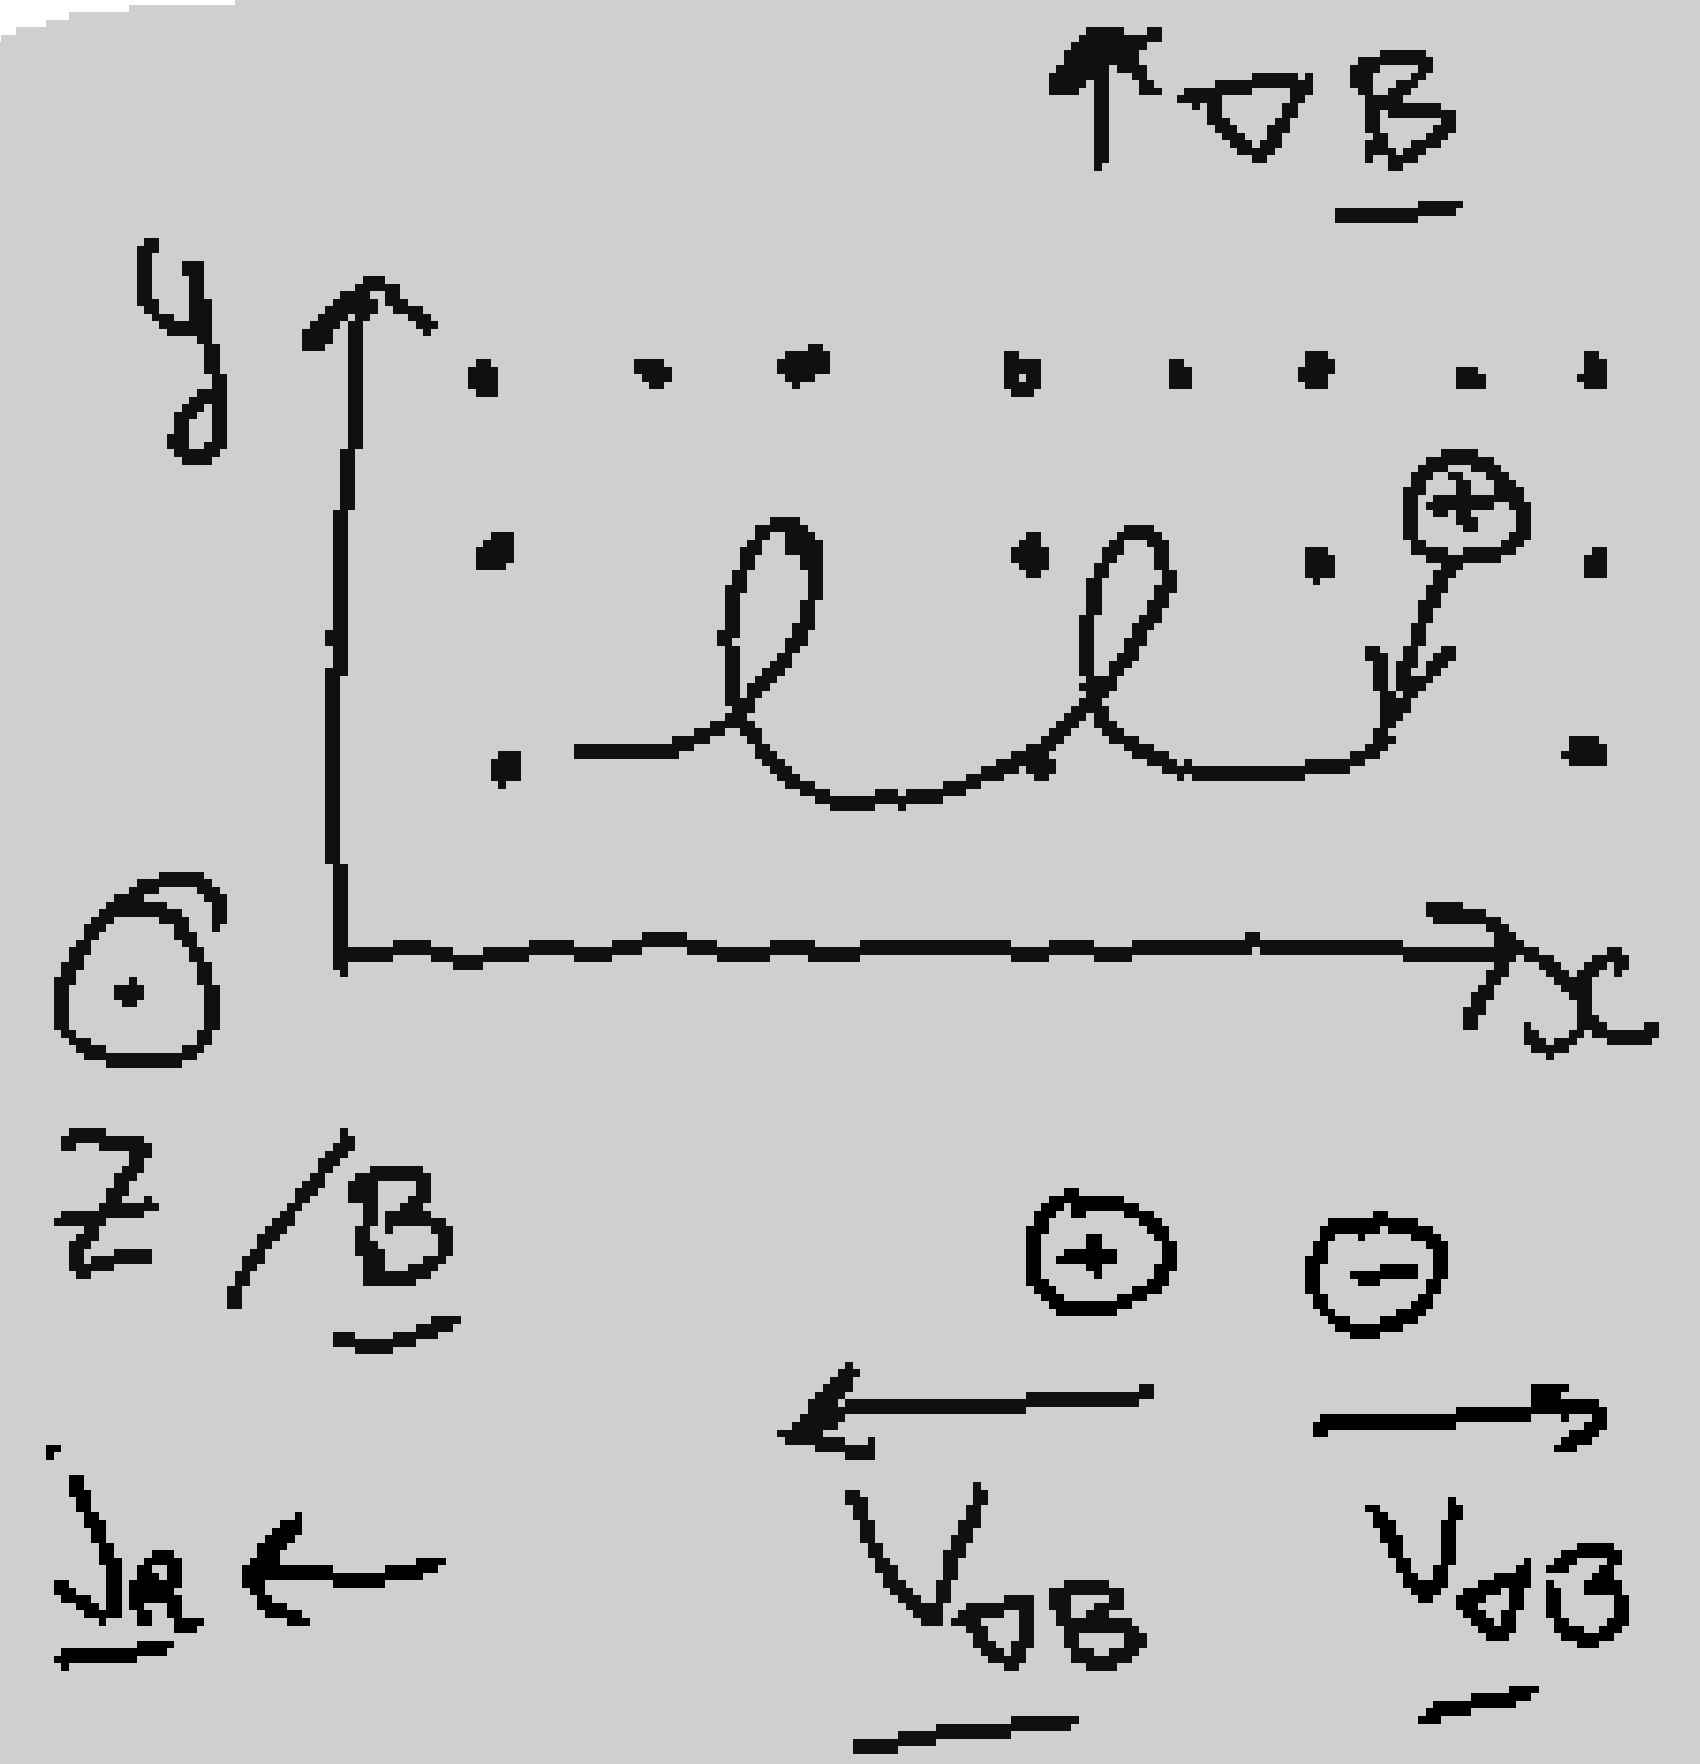
\includegraphics[width=0.2\linewidth]{bilder/gradB.jpg}\label{fig:gradB}
    \caption{\(\nabla\gf{B}\)-drift of ions and electrons.}
\end{figure}
This drift is dependant on charge, and from it we get a current, for instance \(\gf{j}_R~\sim \)~magnetic ring current. This is a current that runs in the westward direction.

\subsection{Curvature \(\gf{B}\)-drift}
A third drift we will look at is due to the curvature of the magnetic field lines, hence the name curvature \(B\)-drift. Let \(\gf{R}_c\) be the radius of a circle made up from the curving magnetic field lines. Motion parallel to these lines will then be described by
\begin{equation*}
    \gf{a}_{\vert\vert}=\frac{v^2_{\vert\vert}}{\gf{R_c}}
\end{equation*}
This give the centrifugal force
\begin{equation*}
    \gf{F}_{cf}=m\gf{a}_{\vert\vert}=m\frac{v^2_{\vert\vert}}{R_c^2}\gf{R}_c
\end{equation*}
This give the curvature drift when we plug this into \cref{eq:gen_v_drift} as
\coloredeq{eq:c_drift}{\gf{u}_{g}=m\frac{v^2_{\vert\vert}}{R_c^2}\frac{\gf{R}_c\times\gf{B}}{qB^2}}
Both \(\gf{u}_{\nabla B}\) and \(\gf{u}_{g}\) in \cref{eq:grad_drift,eq:c_drift} adds to the ring current.
\begin{figure}[t]
    \centering
    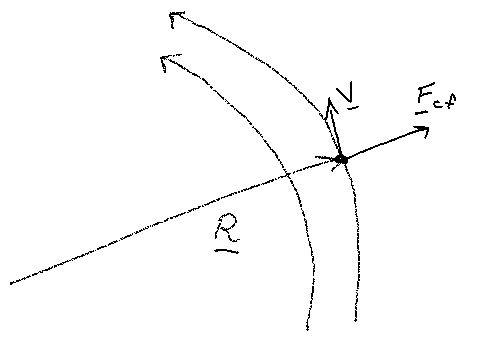
\includegraphics[width=.4\linewidth]{bilder/curve_drift.png}\label{fig:curve_drift}
    \caption{Curvature drift}
\end{figure}
\begin{figure}[t]
    \centering
    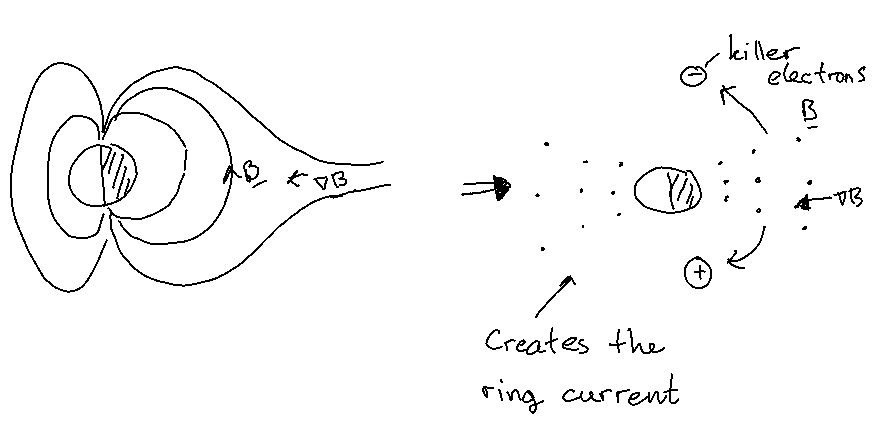
\includegraphics[width=.6\linewidth]{bilder/ring_current.png}\label{fig:ring_current}
    \caption{Ring current}
\end{figure}

\subsection{Magnetic momentum}
The magnetic moment is a quantity that will stay constant even though the energy changes, if the field changes slowly enough. Slowly enough means that the field changes encountered by the particle within a single gyration orbit will be small compared with the initial field. The magnetic moment is defined as \(\mu=IA\) where \(I=\Delta Q/\Delta t=q\omega_c/2\pi=q^2B/2\pi m\) is the current and \(A=\pi r_c^2=\pi mv_\perp/qB\) is the area spanned out by the gyro motion. Plugging the current and the area into the expression for magnetic momentum gives
\coloredeq{eq:magnetic_moment}{\mu=\frac{1}{2}\frac{mv_\perp^2}{B}}
This is known as the \emph{first magnetic invariant}. If we look at the magnetic moment at some point \(E\) along a magnetic field line, we may write the perpendicular component of the velocity in terms of a sine function with argument \(\alpha \), where \(\alpha \) is the angle off the magnetic field line.
\begin{align}
    \mu_E&=\frac{1}{2}\frac{mv_\perp^2}{B_E}\notag \\
    &=\frac{1}{2}\frac{mv^2}{B_E}\sin^2\alpha
\end{align}
\begin{align}
    \mu_M&=\frac{1}{2}\frac{mv_\perp^2}{B_M}\notag \\
    &=\frac{1}{2}\frac{mv^2}{B_M}
\end{align}
where the subscript \(M\) defines the mirror point where we only have a perpendicular velocity component. Since the magnetic moment is conserved we can compare these two to obtain
\begin{align*}
    \mu_E&=\mu_M\\
    \frac{1}{2}\frac{mv^2}{B_E}\sin^2\alpha&=\frac{1}{2}\frac{mv^2}{B_M}
\end{align*}
\begin{equation}
    B_M=\frac{B_E}{\sin^2\alpha}
\end{equation}
and we see how the strength of the magnetic field varies due to them converging when you move closer to the pole. If the angle at point \(E\) is such that \(B_M\) can never get big enough, the particle is lost down to the atmosphere, from which we can define a loss cone as illustrated in \cref{fig:loss_cone}.
\begin{figure}[t]
    \centering
    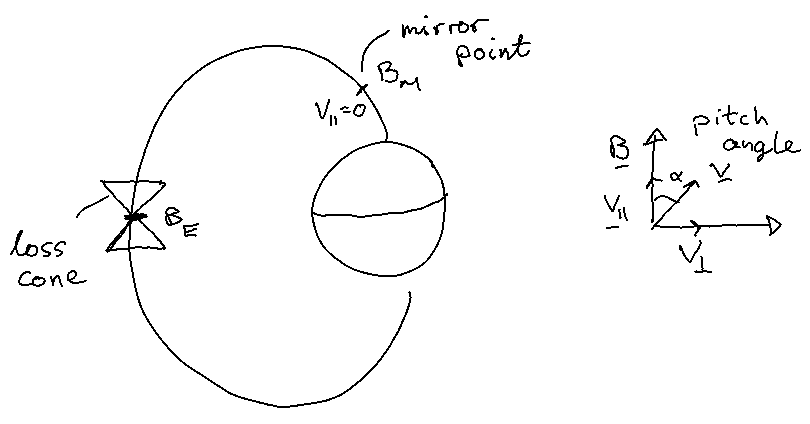
\includegraphics[width=.6\linewidth]{bilder/loss_cone.png}
    \caption{Loss cone}\label{fig:loss_cone}
\end{figure}

\section{Collection of particles}
We will now move on from just describing the motion on one single particle by considering collections of particles. It is handy to introduce the phase space function \(f(\gf{r},\gf{v},t)\)
\begin{align*}
    \gf{r}&=(x,y,z)\\
    \gf{v}&=(v_x,v_y,v_z)\\
    \text{d}\gf{v}\text{d}\gf{r}&=\text{d}v_x\text{d}v_y\text{d}v_z\text{d}x\text{d}y\text{d}z
\end{align*}
From this function you can get information from looking at the different orders of momentum. The \emph{zeroth order momentum} give the number density
\begin{equation*}
    n(\gf{r},t)=\int_{-\infty}^\infty f(\gf{r},\gf{v},t)\text{d}\gf{v}
\end{equation*}
which is related to the mass density \(\rho=nm_i\). The \emph{first order momentum} will give the average velocity of your distribution
\begin{equation*}
    \gf{u}(\gf{r},t)=\overline{\gf{v}(\gf{r},t)}=\frac{\int_{-\infty}^\infty vf(\gf{r},\gf{v},t)\text{d}\gf{v}}{\int_{-\infty}^\infty f(\gf{r},\gf{v},t)\text{d}\gf{v}}
\end{equation*}
while the \emph{second order momentum} give the average energy
\begin{equation*}
    E=\frac{1}{2}m\overline{\gf{v}^2(\gf{r},t)}=\frac{\int_{-\infty}^\infty v^2f(\gf{r},\gf{v},t)\text{d}\gf{v}}{\int_{-\infty}^\infty f(\gf{r},\gf{v},t)\text{d}\gf{v}}
\end{equation*}

\subsection{Maxwellian distribution}
For a uniform, isotropic, and stationary system/plasma, the phase space distribution function reduces to a function of velocity only, often described by a Maxwellian distribution.
\begin{equation*}
    f(v_x)=Ae^{-\frac{1}{2}m{(v_x-u_x)}^2/kT}
\end{equation*}
where \(A\) is the normalization constant. The number density will be
\begin{align*}
    n_s&=A\int_{-\infty}^\infty e^{-\frac{1}{2}m{(v_x-u_x)}^2/kT}\text{d}v_x,\quad a=\sqrt{\frac{m}{2kT}}(v_x-u_x),\text{d}a=\sqrt{\frac{m}{2kT}}\text{d}v_x\\
    &=A\sqrt{\frac{2kT}{m}}\int_{-\infty}^\infty e^{-a^2}\text{d}a\\
    &=A\sqrt{\frac{2kT}{m}}\sqrt{\pi}
\end{align*}
\begin{equation*}
    \therefore A=n\sqrt{\frac{m}{2\pi kT}}
\end{equation*}

\begin{txboxed}
\textbf{ASIDE:} If we look at a point from different places, say Longyearbyen and Tromsø, we may write up the phase space function with the velocity decomposed. We get the bi-Maxwellian distribution
\begin{equation*}
    f(r,t)=A'\exp\left[-\frac{1}{2}\frac{m{(v_{\vert\vert}-u_{\vert\vert})}^2}{kT_{\vert\vert}}\right]\exp\left[-\frac{1}{2}\frac{m{(v_{\perp}-u_{\perp})}^2}{kT_\perp}\right]
\end{equation*}
\end{txboxed}